\documentclass[a4paper]{article}
\usepackage{import}
\usepackage{graphicx}
\usepackage{float}
\usepackage{pgfplots}
\usepackage{listings}
\usepackage{enumitem}
\usepackage{textcomp}
\usepackage{tikz}
\usetikzlibrary{decorations.pathreplacing} % for angle arc
\usetikzlibrary{angles, quotes, calc, positioning, trees} % for drawing angles
\pgfplotsset{compat=1.18,width=10cm}
\usepackage{tikz-cd}
\usepackage{booktabs}
\usepackage{cancel}
\usepackage{amsmath}
\usepackage{minted}
\usepackage{csquotes}
\usepackage{gensymb}
\usepackage{forest}
\usepackage{amsthm}
\usepackage{amssymb}
\usepackage{fontawesome} 
\usepackage{varwidth}
\usepackage{pgfplots}
\usepackage{lipsum}
\usepackage{mdframed} 
\usepackage{color}   
\usepackage{hyperref}
\newmdtheoremenv{theo}{Theorem}
\usepackage{mathtools}
\DeclarePairedDelimiter\ceil{\lceil}{\rceil}
\DeclarePairedDelimiter\floor{\lfloor}{\rfloor}

\hypersetup{
    colorlinks=true, %set true if you want colored links
    linktoc=all,     %set to all if you want both sections and subsections linked
    linkcolor=black,  %choose some color if you want links to stand out
}

% Define theorem styles
\newtheorem{theorem}{Theorem}[section]    % Theorems numbered within sections
\newtheorem{lemma}[theorem]{Lemma}        % Lemmas use the same counter as theorems
\newtheorem{corollary}[theorem]{Corollary} % Corollaries use the same counter as theorems
\newtheorem{proposition}[theorem]{Proposition} % Proposition uses the same counter
\newtheorem{property}[theorem]{Property}
\theoremstyle{definition}
\newtheorem{definition}[theorem]{Definition} % Now uses the same counter as theorems


% Remark-style theorem
\theoremstyle{remark}
\newtheorem{remark}[theorem]{Remark}

% Boxed environment for theorems
\newmdenv[
  linewidth=0.8pt,
  roundcorner=5pt,
  linecolor=black,
  backgroundcolor=white!5,
  skipabove=\baselineskip,
  skipbelow=\baselineskip,
  innerleftmargin=10pt,
  innerrightmargin=10pt,
  innertopmargin=5pt,
  innerbottommargin=5pt
]{thmbox}

% Custom proof environment (also boxed)
\renewenvironment{proof}[1][Proof]{%
  \begin{mdframed}[linewidth=0.8pt, roundcorner=5pt, linecolor=black, skipabove=\baselineskip, skipbelow=\baselineskip, innertopmargin=5pt, innerbottommargin=5pt]%
  \noindent\textbf{#1. }%
}{%
  \end{mdframed}%
}

% Redefine theorem environments to use thmbox
\let\oldtheorem\theorem
\renewenvironment{theorem}{\begin{thmbox}\begin{oldtheorem}}{\end{oldtheorem}\end{thmbox}}

\let\oldlemma\lemma
\renewenvironment{lemma}{\begin{thmbox}\begin{oldlemma}}{\end{oldlemma}\end{thmbox}}

\let\oldcorollary\corollary
\renewenvironment{corollary}{\begin{thmbox}\begin{oldcorollary}}{\end{oldcorollary}\end{thmbox}}

\let\oldproposition\proposition
\renewenvironment{proposition}{\begin{thmbox}\begin{oldproposition}}{\end{oldproposition}\end{thmbox}}

\let\oldproperty\property
  \renewenvironment{property}{\begin{oldproperty}}{\end{oldproperty}}


% Reference shortcuts
\newcommand{\thmref}[1]{Theorem~\ref{#1}}
\newcommand{\lemref}[1]{Lemma~\ref{#1}}
\newcommand{\corref}[1]{Corollary~\ref{#1}}
\newcommand{\propref}[1]{Property~\ref{#1}} 

% To customize QED symbol
\renewcommand{\qedsymbol}{$\blacksquare$}

\usetikzlibrary{decorations.pathreplacing} % for angle arc
\usetikzlibrary{angles, quotes, calc} % for drawing angles

\usepackage{color}   %May be necessary if you want to color links
\usepackage{hyperref}
\hypersetup{
    colorlinks=true, %set true if you want colored links
    linktoc=all,     %set to all if you want both sections and subsections linked
    linkcolor=black,  %choose some color if you want links to stand out
}

\usepackage{xcolor}
\usepackage[most]{tcolorbox}


% Define a custom tcolorbox environment for examples
\newtcolorbox{examplebox}[2][]{
  colback=blue!5!white,
  colframe=blue!30!black,
  title=#2,
  boxrule=0mm,
  fonttitle=\bfseries,
  width=\textwidth,
  breakable,
  #1
}

\newtcolorbox{definizione}[2] {
  colback=green!5!white,
  colframe=green!30!black,
  title=#2,
  boxrule=0mm,
  fonttitle=\bfseries,
  width=\textwidth,
  breakable,
  #1
}

\definecolor{codegreen}{rgb}{0,0.6,0}
\definecolor{codegray}{rgb}{0.5,0.5,0.5}
\definecolor{codepurple}{rgb}{0.58,0,0.82}
\definecolor{backcolour}{rgb}{0.95,0.95,0.92}

\lstdefinestyle{mystyle}{
    backgroundcolor=\color{backcolour},   
    commentstyle=\color{codegreen},
    keywordstyle=\color{magenta},
    numberstyle=\tiny\color{codegray},
    stringstyle=\color{codepurple},
    basicstyle=\ttfamily\footnotesize,
    breakatwhitespace=false,         
    breaklines=true,                 
    captionpos=b,                    
    keepspaces=true,                 
    numbers=left,                    
    numbersep=5pt,                  
    showspaces=false,                
    showstringspaces=false,
    showtabs=false,                  
    tabsize=2
}

\lstset{style=mystyle}

\makeatletter
\renewcommand*\env@matrix[1][*\c@MaxMatrixCols c]{%
  \hskip -\arraycolsep
  \let\@ifnextchar\new@ifnextchar
  \array{#1}}
\makeatother

\title{Operating Systems Writeup}
\author{SETU - South East Technological University\\Imbriani Paolo - W20114452\\Professor Micheal McMahon}

\begin{document}

\begin{figure}
    \centering
    
\includegraphics[width=0.6\textwidth]{SETU.png}
    \label{fig:centered-image}
\end{figure}

\maketitle 

\pagebreak

\tableofcontents

\pagebreak

\section{Practical 1 -  Commands}


\textcolor{green!50!black}{
Taking a selection of Windows CLI commands from those given below, use the online help to
examine the various options and arguments, and try them out.\\
You're required carefully to write two A4 pages (Times 12 point or equivalent size) detailing your experiments with different options for between six and ten different commands.
To get the online help for a command, type command /?\\
e.g.\\
dir /?\\
prompt\\
mkdir\\
color\\
title\\
tree\\
type\\
ver\\
print\\
xcopy\\
Type help at the windows command line prompt to see some more instructions
}

\begin{itemize}
    \item Prompt - The prompt command is used to customize the text that appears before the cursor in the command prompt.
\begin{lstlisting}[language=bash]
prompt MyPrompt$G
\end{lstlisting}
This changes the prompt to MyPrompt$>$. The \$G represents the $>$ symbol.
\item Mkdir - The mkdir command is used to create a new directory.
\begin{lstlisting}[language=bash]
mkdir MyDirectory
\end{lstlisting}
This creates a new directory called MyDirectory. To create a folder inside another folder:
\begin{lstlisting}[language=bash]
mkdir MyDirectory\MySubDirectory
\end{lstlisting}
\item Color - The color command is used to change the color of the text and background in the command prompt.
\begin{lstlisting}[language=bash]
color 0A
\end{lstlisting}
This sets a black background (0) with green text (A).
To reset to default:
\begin{lstlisting}[language=bash]
color
\end{lstlisting}
To see all the available colors:
\begin{lstlisting}[language=bash]
color /?
\end{lstlisting}
\item Title - The title command is used to change the title of the command prompt window.
\begin{lstlisting}[language=bash]
title MyTitle
\end{lstlisting}
This changes the title of the command prompt window to MyTitle.
\item Tree - The tree command is used to display a graphical representation of the directory structure.
\begin{lstlisting}[language=bash]
tree
\end{lstlisting}
And it will output something like this:
\begin{figure}[H]
    \centering
    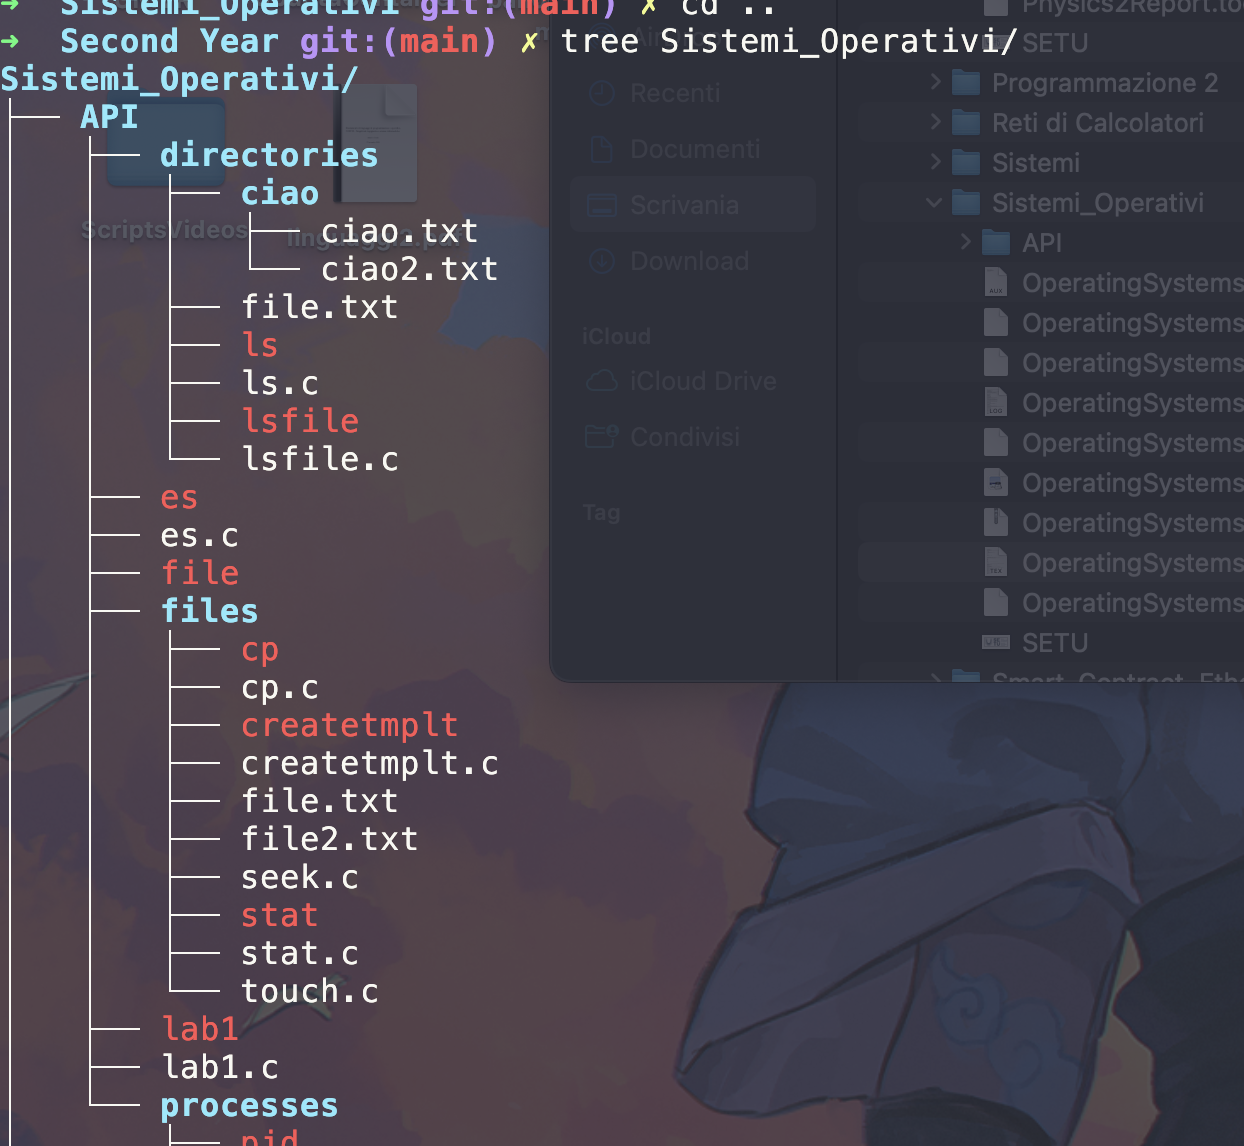
\includegraphics[width=0.6\textwidth]{treeEx.png}
    \label{fig:centered-image}
\end{figure}
Displays a simple tree structure of folders in the current directory. To include all files in the display:
\begin{lstlisting}[language=bash]
tree /f
\end{lstlisting}
The /F option lists all files along with the folder structure.
\item Type - The type command is used to display the contents of a text file.   
\begin{lstlisting}[language=bash]
type MyFile.txt
\end{lstlisting}
This displays the contents of the file MyFile.txt. Useful for quickly viewing small text files without opening them.
\item Ver - The ver command is used to display the version of the operating system.
\begin{lstlisting}[language=bash]
ver
\end{lstlisting}
This displays the version of the operating system.


\end{itemize}
\textcolor{green!50!black}{What’s the purpose of the first line - @ECHO OFF? Remove it and see the
effect}

\begin{lstlisting}[language=bash]
@ECHO OFF
ECHO Please insert a USB memory stick
PAUSE
COPY *.txt I:\
ECHO BACKUP COMPLETE
\end{lstlisting}
\begin{itemize}
    \item @ECHO OFF → Hides command execution lines for cleaner output.
    \item ECHO → Displays messages on the screen.
    \item PAUSE → Waits for the user to press a key before continuing.
    \item COPY *.txt I:\ → Copies all .txt files from the current folder to the USB drive (assuming it's drive I:).
    \item ECHO BACKUP COMPLETE → Displays a completion message.
\end{itemize}
The first line, @ECHO OFF, is used to prevent the command prompt from displaying each command as it executes.
\begin{lstlisting}[language=bash]
C:\Users\YourName\Desktop> ECHO Please insert a USB memory stick
Please insert a USB memory stick

C:\Users\YourName\Desktop> PAUSE
Press any key to continue . . .

C:\Users\YourName\Desktop> COPY *.txt I:\
3 file(s) copied.

C:\Users\YourName\Desktop> ECHO BACKUP COMPLETE
BACKUP COMPLETE
\end{lstlisting}



\end{document}